\documentclass[tikz,border=5pt]{standalone}
\usepackage{pgfplots}\pgfplotsset{compat=1.18}
\definecolor{tramU}{HTML}{365FB3}\definecolor{tramDos}{HTML}{0F766E}\definecolor{tramTres}{HTML}{D97706}\definecolor{punt}{HTML}{B91C1C}
\begin{document}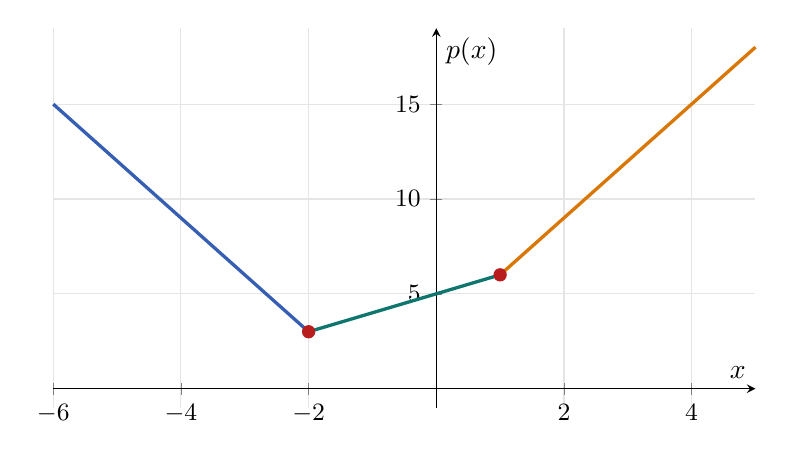
\begin{tikzpicture}
\begin{axis}[width=10.5cm,height=6.4cm,axis lines=middle,xmin=-6,xmax=5,ymin=-1,ymax=19,
 xlabel={$x$},ylabel={$p(x)$},grid=major,grid style={black!10},tick label style={font=\small},clip=false]
 \addplot[tramU,very thick,domain=-6:-2]{-3*x-3};\addplot[tramDos,very thick,domain=-2:1]{x+5};\addplot[tramTres,very thick,domain=1:5]{3*x+3};
 \addplot[only marks,mark=*,mark size=2.2pt,punt] coordinates {(-2,3)(1,6)};
\end{axis}\end{tikzpicture}\end{document}
